\documentclass{article}
\usepackage{graphicx, color}


\setlength{\textwidth}{6.5in}
\setlength{\textheight}{8.0in}
\setlength{\oddsidemargin}{0in}
\setlength{\evensidemargin}{0in}
\setlength{\parskip}{2ex}
\setlength{\parindent}{0in}

%To display answers, replace "white" with "red" here;
\newcommand{\answer}[1]{\color{red}#1}

\begin{document}
\pagestyle{myheadings}\markright{
CU Boulder \hspace{0.5in} MATH 2510 - Introduction to Statistics }

\begin{center}
\textbf{\underbar{In-class Worksheet 11}}
\end{center}

Today's worksheet is an in-class activity with the goal of simulating a sampling distribution of sample means. The first part of the activity is for each of you to generate a list of sample means. After the data is gathered, the second part directs you to use the results of the entire class to analyze the outcome.

\textbf{PART 1}

\begin{enumerate}

\item Attached to this page is a copy of a random number table for the population of digits \{0, 1, 2, 3, 4, 5, 6, 7, 8, 9\}. Assuming that this random distribution is uniform:

	\begin{enumerate}
	
	\item What is the population mean of the digits? 
	
	{\answer Since the frequency of all digits is equally weighed, $\mu = \frac{0+1+2+3+4+5+6+7+8+9}{10} = 4.5$.
	}
	
	\item What is the population standard deviation of the digits? 
	
	{\answer This could be done by hand (like the mean just was) or entering $L_1=\{0, 1, 2, 3, 4, 5, 6, 7, 8, 9\}$, \texttt{1-VarStats} indicates that $\sigma = 2.872281323$.
	} 
	\end{enumerate}
	
\item Repeat the following steps 10 times. In the end, you will have generated 10 different sample means. Please do NOT simply copy a classmate's values on this part, but please do your own work so that you really are generating your own list of sample means. 

	\begin{enumerate}
	
	\item {\em Randomly} select a spot on the random number table.
	
	\item Write down the next 10 digits listed from that spot horizontally (if you reach the end of a row, wrap around to the start of the next row to complete your list of 10). 
	
	\item Compute the mean of that sample of 10 random digits. 
	
	\end{enumerate}

\begin{center}	

\begin{tabular}{|c|c||c|}
\hline
Sample & List of 10 digits & Sample mean \\
\hline
1 & \hspace{3in} & \hspace{1in} \\
&&\\ \hline
2 & \hspace{3in} & \hspace{1in} \\
&&\\ \hline
3 & \hspace{3in} & \hspace{1in} \\
&&\\ \hline
4 & \hspace{3in} & \hspace{1in} \\
&&\\ \hline
5 & \hspace{3in} & \hspace{1in} \\
&&\\ \hline
6 & \hspace{3in} & \hspace{1in} \\
&&\\ \hline
7 & \hspace{3in} & \hspace{1in} \\
&&\\ \hline
8 & \hspace{3in} & \hspace{1in} \\
&&\\ \hline
9 & \hspace{3in} & \hspace{1in} \\
&&\\ \hline
10 & \hspace{3in} & \hspace{1in} \\
&&\\ \hline
\end{tabular}

\end{center}

\end{enumerate}

\textbf{PART 2}

\begin{enumerate}

\item Looking at the list of sample means, there should be a variety of values, but they are not uniformly distributed. What is the shape of the distribution for the sample means?

{\answer This will certainly vary from section to section, but the distributions should be roughly single-mound, symmetric.
} 

\item What is the mean of the sample means? 

{\answer Again, the specific answers will vary from section to section, but the outcome should be close to the population mean of $4.5$.
} 

\item What is the standard deviation of the sample means? 

{\answer Again, the specific answers will vary from section to section, but the outcome should not be too far from $\frac{2.872281323}{\sqrt{(10)}} \approx 0.9082951$.
} 

\item In Section 6.5, one of the most critical theorems in statistics is introduced; the Central Limit Theorem. Essentially it says that a sampling distribution for sample means (where the sample size for all samples is $n$) will have a distribution close to a normal distribution. Further, the mean of the sample means will equal the population mean $\mu$ and the standard deviation of the sample means will equal $\frac{\sigma}{\sqrt{(n)}}$. How did the simulation the class do match up to the theorem? 

	\begin{enumerate}
	
	\item Was the shape of the distribution of sample means approximately normal? 
	
	{\answer Answers will vary.
	} 
	
	\item Was the mean of the sample means close the the population mean $\mu$? 
	
	{\answer Answers will vary.
	} 
	
	\item What was the sample size for our sample means? 
	
	{\answer $n = 10$ 
	} 
	
	\item Was the standard deviation of the sample means close to the value $\frac{\sigma}{\sqrt{(n)}}$? 
	
	{\answer Answers will vary, but $\frac{\sigma}{\sqrt{(n)}} = \frac{2.872281323}{\sqrt{(10)}} \approx 0.9082951$.
	} 
	
	\end{enumerate}
	

\end{enumerate}

\vfill
\pagebreak

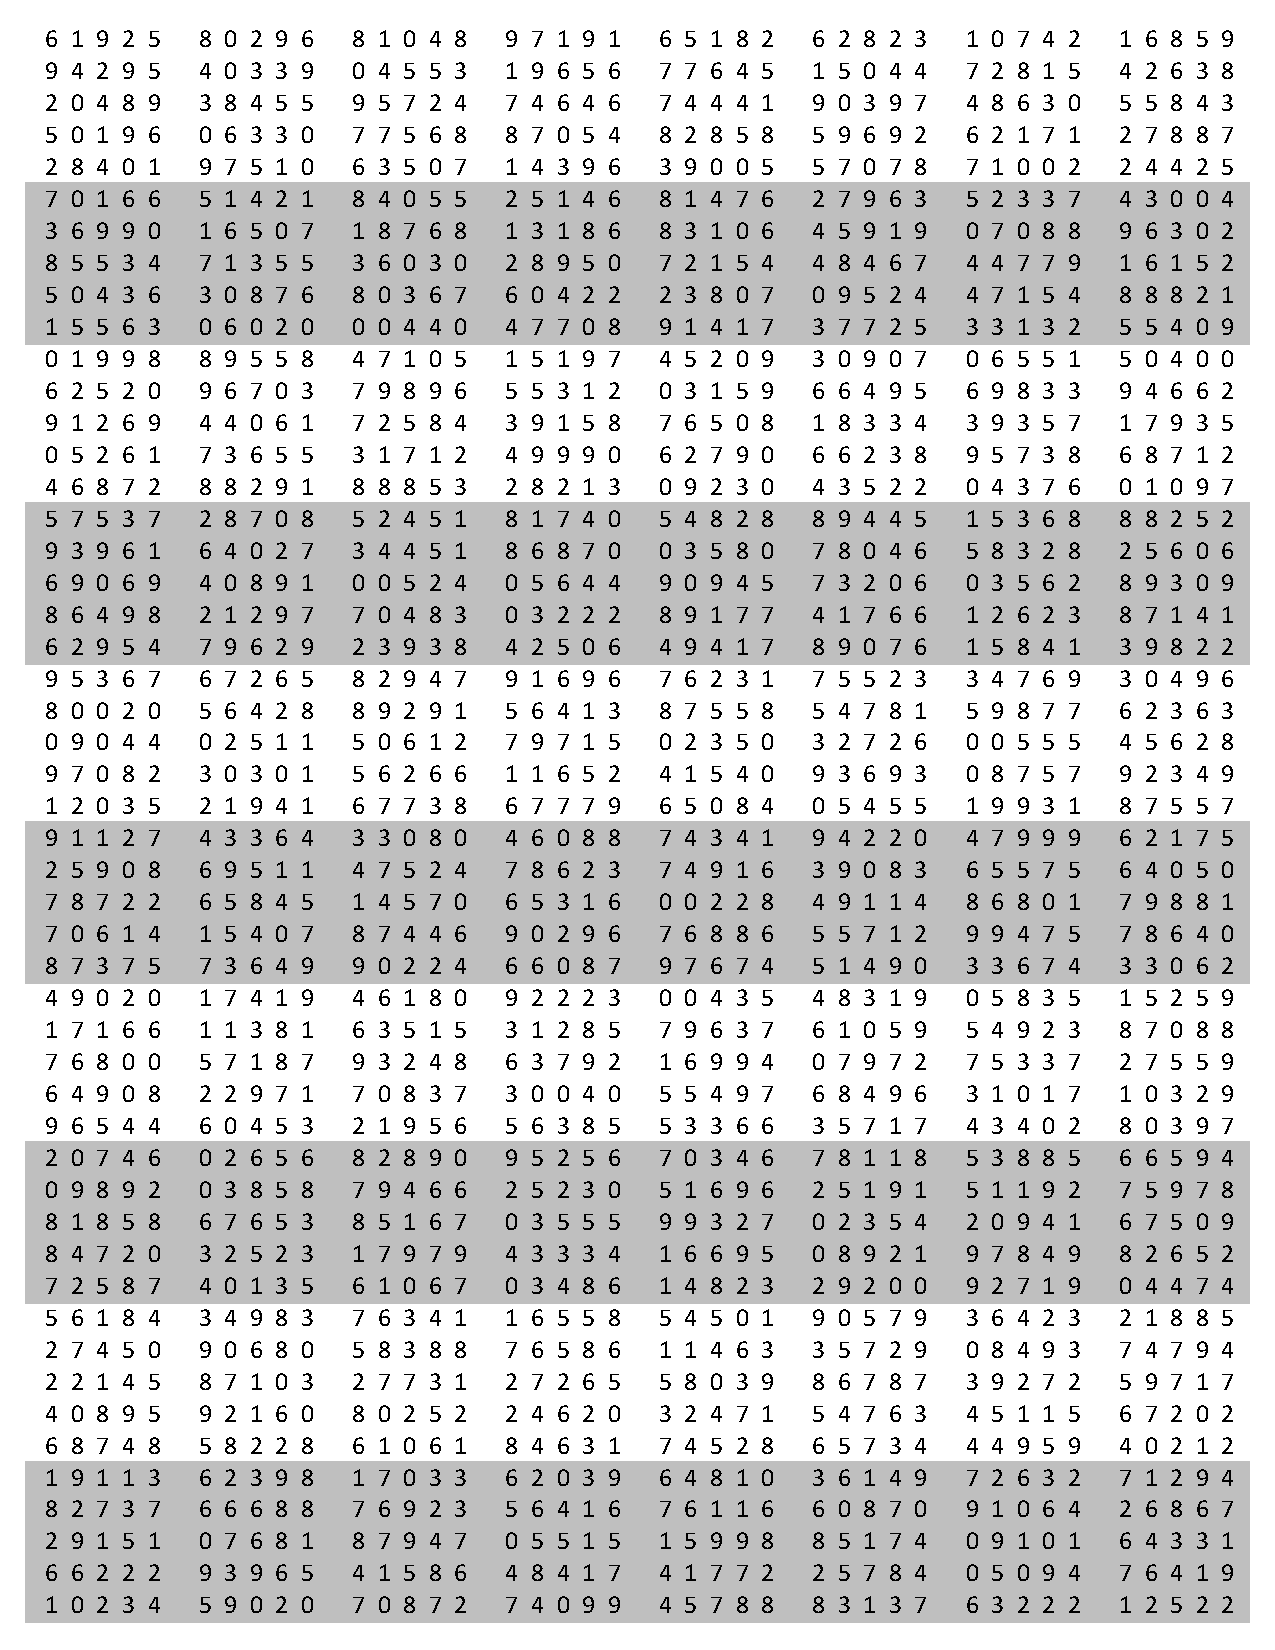
\includegraphics[scale=0.7]{RandNumbers.pdf}


\end{document}

